\documentclass{article}
\usepackage{setspace}
\usepackage{arabtex}
\usepackage{utf8} 
\usepackage{hyperref} 
\usepackage{graphicx}
\usepackage{subcaption}
\usepackage{tabularx}
\usepackage{geometry}
\usepackage{lipsum}
\usepackage{listings}
\usepackage{color}
\usepackage{enumitem}

\definecolor{dkgreen}{rgb}{0,0.6,0}
\definecolor{gray}{rgb}{0.5,0.5,0.5}
\definecolor{mauve}{rgb}{0.58,0,0.82}

\newcounter{magicrownumbers}
\newcommand\rownumber{\stepcounter{magicrownumbers}\arabic{magicrownumbers}}

\lstset{frame=tb,
	language=Java,
	aboveskip=3mm,
	belowskip=3mm,
	showstringspaces=false,
	columns=flexible,
	basicstyle={\small\ttfamily},
	numbers=none,
	numberstyle=\tiny\color{gray},
	keywordstyle=\color{blue},
	commentstyle=\color{dkgreen},
	stringstyle=\color{mauve},
	breaklines=true,
	breakatwhitespace=true,
	tabsize=3
}

\setcounter{tocdepth}{2}
\hypersetup{
	colorlinks,
	citecolor=[rgb]{0,0.5,0.5},
	filecolor=[rgb]{0,0.5,0.5},
	linkcolor=[rgb]{0,0.5,0.5},
	urlcolor=[rgb]{0,0.5,0.5}
}

\date{}
\title{
	Bank Automated Teller Machines \\
	\large Software Engineering (CS385T) Project }

\author{
	\setcode{utf8}
	\RL{ريم علي الغامدي} 
	\\\texttt{437004875}
	\\[3ex]
	\RL{سارة خالد آل حسين} 
	\\\texttt{436006939}
	\\[3ex]
	\RL{شهد الكناني} 
	\\\texttt{437004165}
	\\[3ex]
	\RL{عبير عزت} 
	\\\texttt{436200058}
	\\[3ex]
	\RL{لمياء القحطاني} 
	\\\texttt{437004164}
}

\begin{document}
	
	
	\pagenumbering{gobble}
	\maketitle
	\newpage
	\addcontentsline{toc}{section}{Member Roles}
	
	\def\arraystretch{2}
	\begin{table}[h!]
		\begin{center}
			\caption{Member Roles}
			\begin{tabularx}{\textwidth}{r|c|X}
				\textbf{Name} & 
				\textbf{ID} & 
				\textbf{Responsibility}\\
				\hline
				\RL{ريم علي الغامدي} &
				\texttt{437004875} &
				Transfer
				\\
				\hline
				\RL{سارة خالد آل حسين} &
				\texttt{436006939} &
				Withdraw
				\\
			\hline
				\RL{شهد الكناني} &
				\texttt{437004165} &
				validate
				\\
				\hline
				\RL{عبير عزت} &
				\texttt{436200058} &
				Deposit
				\\
			\hline
				\RL{لمياء القحطاني} &
				\texttt{437004164} &
				Retrieve
				\\
				
			\end{tabularx}
		\end{center}
	\end{table}

	\newpage
	\pagenumbering{arabic}
	\addcontentsline{toc}{section}{Table of Contents}\tableofcontents
	\newpage	
	\doublespacing
	\newpage
	
	

	\section{Introduction}
		The ATM (Automated Teller Machine) is a machine that helps clients access their money that’s in their bank accounts and do transactions on it. It does so when the client inserts a plastic ATM card with a verification PIN into this machine and the machine just retrieves the client’s account information from the bank itself. The clients can do multiple transactions on the money they own in the bank including allowing them to specifically to see the amount of money they have, add their cash into their accounts, transfer money to some other account, and take some cash out, all with the use of that card. The system can print a receipt at the end of each transaction if the user wishes\cite{atm}.
	\subsection{Purpose}
		\begin{enumerate}
			\item Making transactions easier for clients
		    \item Making transactions more accessible to clients, since the ATMs are at remote locations closer to the client
		    \item Saving time so that clients don’t have to have actual interactions with bank staff
		    \item Reducing the number of staff that have to be at a branch (clients can do the transactions themselves)
		    \item Allowing the clients to “carry around” their money with them in a safer way, without it being in cash form
		\end{enumerate}
  
	\subsection{Scope}
	The area that the system is concerned with is financial; it is monetary transactions that banks will allow clients to carry out on their own. This system shall help with the following transaction: deposit, withdraw, retrieving info and transfer. This system is not concerned with changing PIN, making new account or paying bills.
	\subsection{Generic Software Model}
	The model we are going to use to develop the ATM system is the waterfall model. It is the most suitable one because the requirements of the system were very clear from the beginning (allowing remote monetary transactions that included balance inquiry, money deposit, money transfer, and money withdrawal) and are not going to change or increase with time, and because we can finish from one phase and start the other without them overlapping them; i.e. we can finish collecting and verifying all the required functionalities, then designing each of them separately and finishing from all their design process, then implementing their designs as codes, integrating them, and finally deploying them \cite{waterfall}.
	\section{Requirement Specifications}
	\subsection{Functional Requirements}


	\begin{enumerate}[label*=\arabic*.]
		\item The ATM shall validate the user.
		\item The user shall be able to retrieve account information.	
		\item The user shall be able to withdraw money.
		\item The user shall be able to deposit money.
		\item The user shall be able to transfer money to another account.
	\end{enumerate}

	\subsection{Non-functional Requirements}
	\begin{enumerate}
		\item The system must be secure.
		\item The system must be available 24H.
	\end{enumerate}

	\newpage\subsection{Functional Requirements Description}
	\setcounter{magicrownumbers}{0}
	\def\arraystretch{2}
	\begin{table}[h!]
		\begin{center}
			\begin{tabularx}{\textwidth}{r|X|X}
				\textbf{ID} & 
				\textbf{Requirement} & 
				\textbf{Description}\\
				\hline
				\rownumber &
				The ATM shall validate the user. &
				ATM should ask for the user card and PIN code, then send these information to the bank to validate the user, if PIN is correct bank sends the user account to the ATM
				\\
				\hline

				\rownumber &
				The user shall be able to retrieve account information. &
				After the user is validated, the user should be able to get account information. Including current balance, debt, number of cards activated, and the last transactions.
				\\
				\hline
				\rownumber &
				The user shall be able to withdraw money. &
				After the user is validated, the user should be able to get withdraw money from account if withdrawn amount is less than the balance.
				\\
				\hline
				\rownumber &
				The user shall be able to deposit money. &
				After the user is validated, the user should be able to deposit money into account if money is validated to be real and undamaged.
				\\
				\hline
				\rownumber &
				The user shall be able to transfer money to another account. &
				After the user is validated, the user should be able to transfer money from account to any other account as long as IBAN entered is correct and amount transferred is less than the balance.
				\\	
			\end{tabularx}
		\end{center}
	\end{table}

	\newpage\subsection{Non-functional Requirements Description}
	\setcounter{magicrownumbers}{0}
	\def\arraystretch{2}
	\begin{table}[h!]
		\begin{center}
			\begin{tabularx}{\textwidth}{r|X|X}
				\textbf{ID} & 
				\textbf{Requirement} & 
				\textbf{Description}\\
				\hline
				\rownumber &
				The system must be secure. &
				The system must be impossible to hack, connection must be secure and data must be encrypted and layered.
				\\
				\hline

				\rownumber &
				The system must be available 24H. &
				The system must never fail or else the user or the bank might lose money.
				\\
			
			\end{tabularx}
		\end{center}
	\end{table}

	\newpage\section{Design}
	\subsection{Validate User}
	\subsubsection{Use Case Scenario}
		\textbf{Use Case Name:}	validate user.
		\newline\textbf{Goal:} to validate the client.
		\newline\textbf{Actors:} customer, Bank. 	
		\newline\textbf{Precondition:} the ATM is free. 	
		\newline\textbf{Primary Scenario:}	
			\begin{enumerate}[label*=\arabic*.]
				\item the system starts to work.
				\item the customer insert the card into the ATM 
				\item ATM ask customer for the PIN code
				\item the customer enters PIN code
				\item the ATM authenticate PIN with the bank
				\item the ATM gets customer's bank account from the bank
			\end{enumerate}
		\textbf{Variant:}\newline	
			\hspace*{5mm}4a. the customer enter wrong PIN code.\newline
			\hspace*{5mm}4b. the user enter the PIN code wrong more than 3 times.

		\newpage\subsubsection{Use Case Diagram}
			\begin{figure}[h!]
			  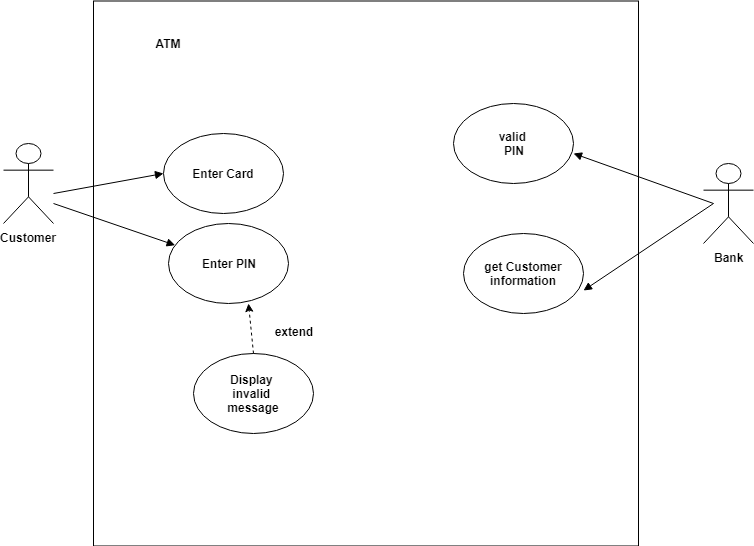
\includegraphics[width=\linewidth]{img/validate_usecase.png}
			\end{figure}

		\newpage\subsubsection{Sequence Diagrams}
		\begin{figure}[h!]
		  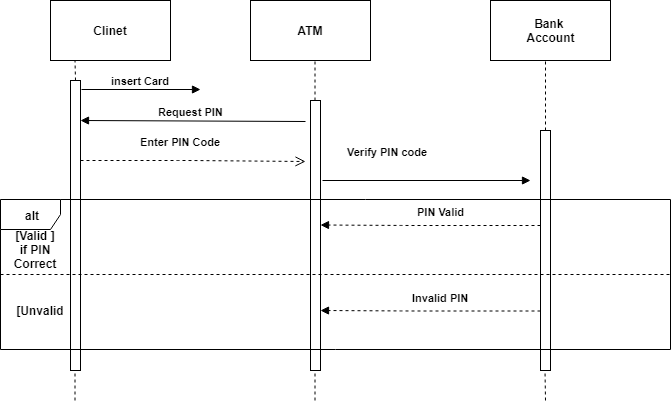
\includegraphics[width=\linewidth]{img/validate_sequence.png}
		\end{figure}

		\newpage\subsubsection{Collaboration Diagram}	
		\begin{figure}[h!]
		  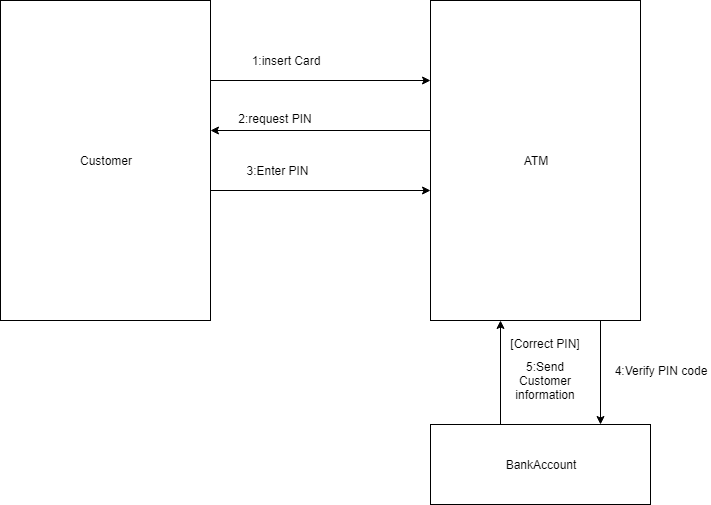
\includegraphics[width=\linewidth]{img/validate_collaboration.png}
		\end{figure}

		\newpage\subsubsection{Activity Diagram}
		\begin{figure}[h!]
			\begin{center}
				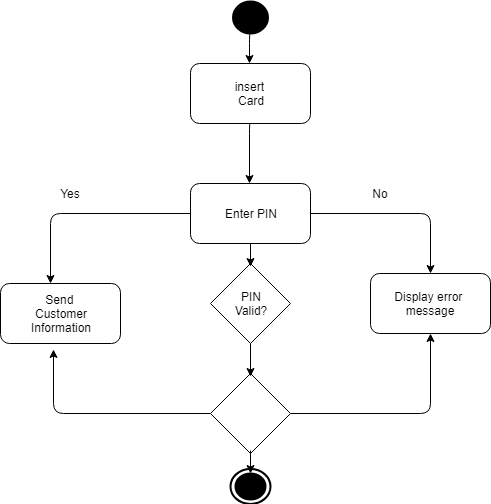
\includegraphics[height=\linewidth]{img/validate_activity.png}
			\end{center}
		\end{figure}

		\newpage\subsubsection{Flow Chart}
		\begin{figure}[h!]
			\begin{center}
				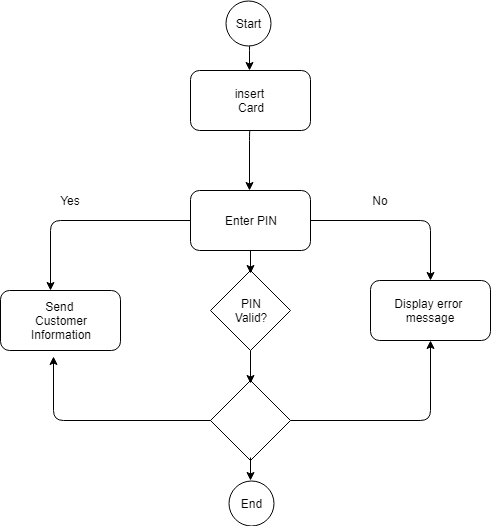
\includegraphics[height=\linewidth]{img/validate_flowchart.png}
			\end{center}
		\end{figure}
	
	
	\newpage\subsection{Retrieve Account Information}
	\subsubsection{Use Case Scenario}
		\textbf{Use Case Name:}	Retrieve info.
		\newline\textbf{Goal:} to check account balance.
		\newline\textbf{Actors:} customer, Bank 	
		\newline\textbf{Precondition:} user is validated 	
		\newline\textbf{Primary Scenario:}	
			\begin{enumerate}[label*=\arabic*.]
				\item ATM shows menu.
				\item user chooses “ Balance Inquiry ”.
				\item ATM prints receipt.
				\item ATM go back to menu.
				\item User quit.
				\item ATM return the card to user.
			\end{enumerate}
		\textbf{Variant:}\newline	
			\hspace*{5mm}*. user may cancel the session ;ATM return card.


		\newpage\subsubsection{Use Case Diagram}
			\begin{figure}[h!]
			  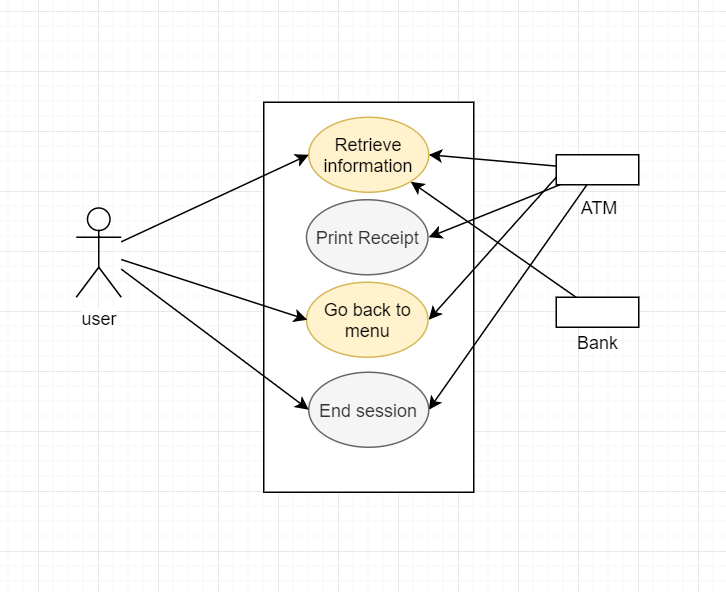
\includegraphics[width=\linewidth]{img/inquiry_usecase.png}
			\end{figure}

		\newpage\subsubsection{Sequence Diagrams}
		\begin{figure}[h!]
		  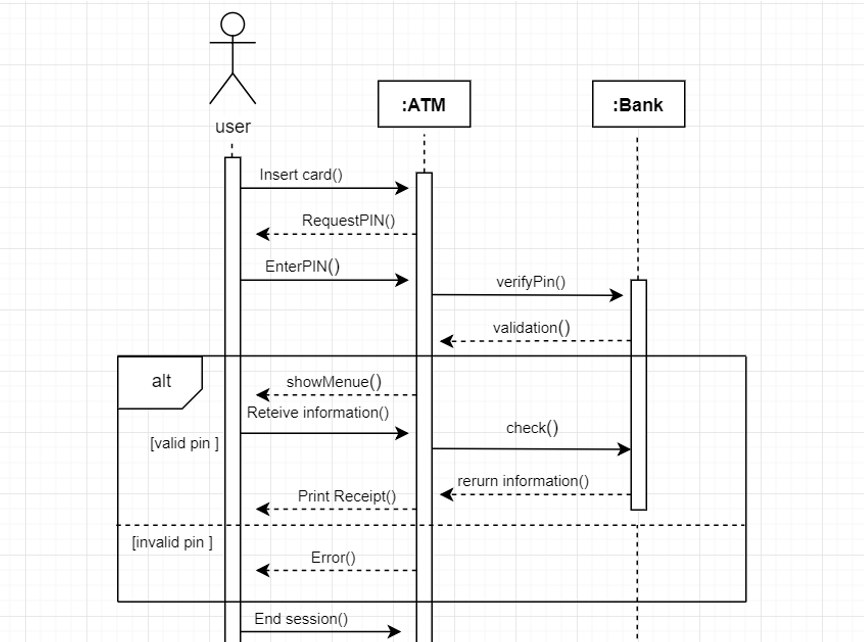
\includegraphics[width=\linewidth]{img/inquiry_sequence.png}
		\end{figure}

		\newpage\subsubsection{Collaboration Diagram}	
		\begin{figure}[h!]
		  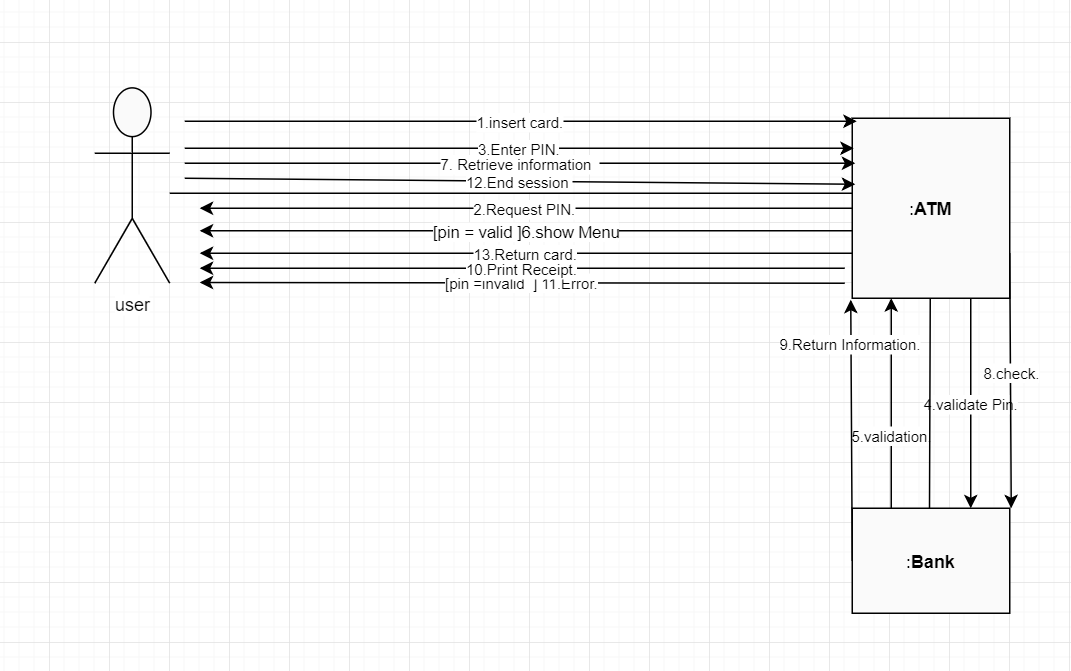
\includegraphics[width=\linewidth]{img/inquiry_collaboration.png}
		\end{figure}

		\newpage\subsubsection{Activity Diagram}
		\begin{figure}[h!]
			\begin{center}
				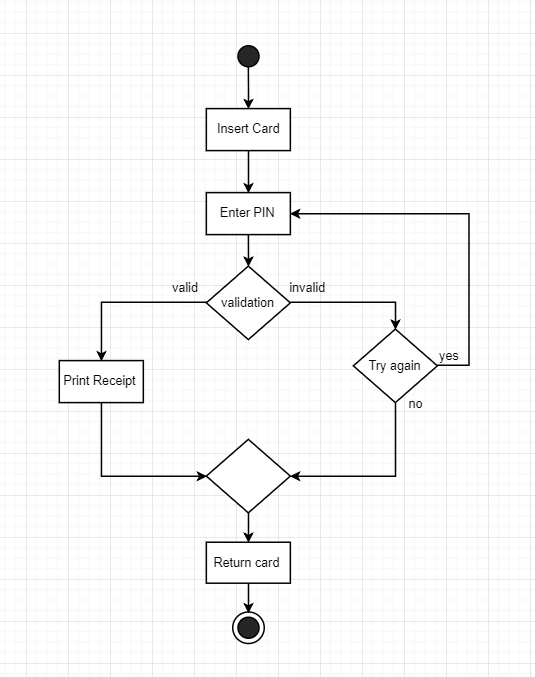
\includegraphics[height=\linewidth]{img/inquiry_activity.png}
			\end{center}
		\end{figure}

		\newpage\subsubsection{Flow Chart}
		\begin{figure}[h!]
			\begin{center}
				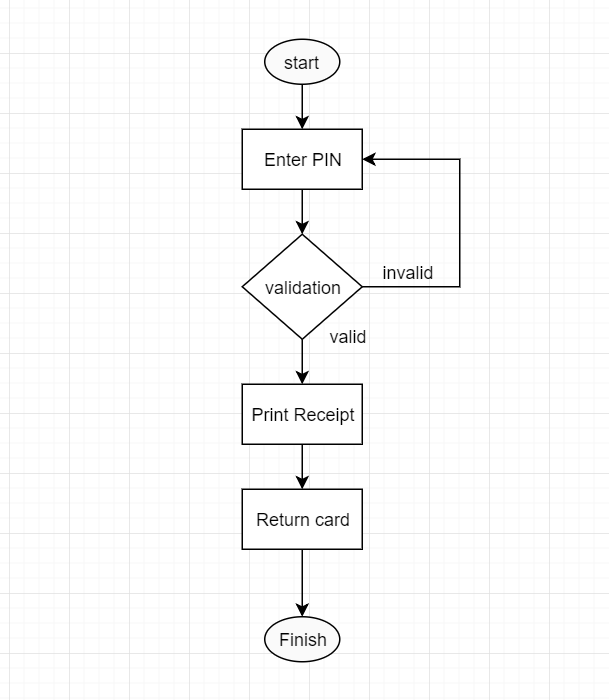
\includegraphics[height=\linewidth]{img/inquiry_flowchart.png}
			\end{center}
		\end{figure}
	
	\newpage\subsection{Withdraw Money}
	\subsubsection{Use Case Scenario}
		\textbf{Use Case Name:} withdraw money.
		\newline\textbf{Goal:} to get money.
		\newline\textbf{Actors:} customer, Bank. 	
		\newline\textbf{Precondition:} user is validated. 	
		\newline\textbf{Primary Scenario:}	
			\begin{enumerate}[label*=\arabic*.]
				\item User insert  card  into ATM machine.
				\item ATM machine request PIN from the user.
				\item The user enter PIN code .
				\item The ATM will verify PIN code entered with saving user account .
				\item ATM machine request amount if PIN is valid .
				\item The user enter the required amount .
				\item Process the transaction in the client account .
				\item ATM machine dispense cash if  the transaction successful .
				\item The ATM ejects  the users card .
			\end{enumerate}
		\textbf{Variant:}\newline	
			\hspace*{5mm}3a. Invalid PIN code entered. Indicate error message. Return step 3.\newline
			\hspace*{5mm}6a. If the amount is unavailable int the user's account. Return step 6.

		\newpage\subsubsection{Use Case Diagram}
			\begin{figure}[h!]
			  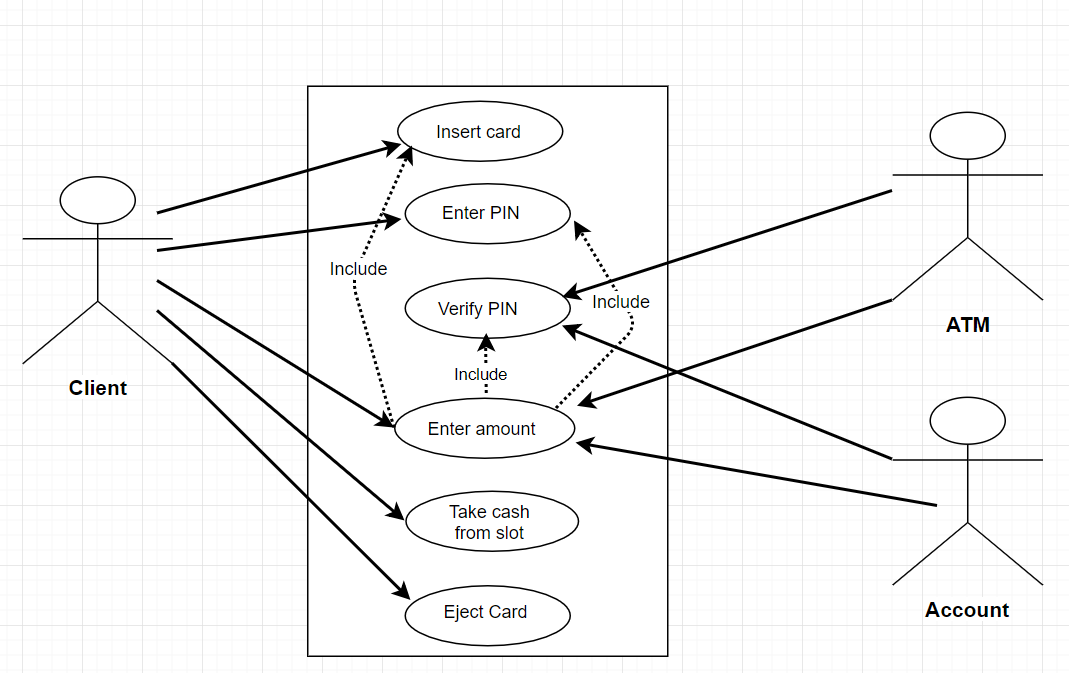
\includegraphics[width=\linewidth]{img/withdraw_usecase.png}
			\end{figure}

		\newpage\subsubsection{Sequence Diagrams}
		\begin{figure}[h!]
		  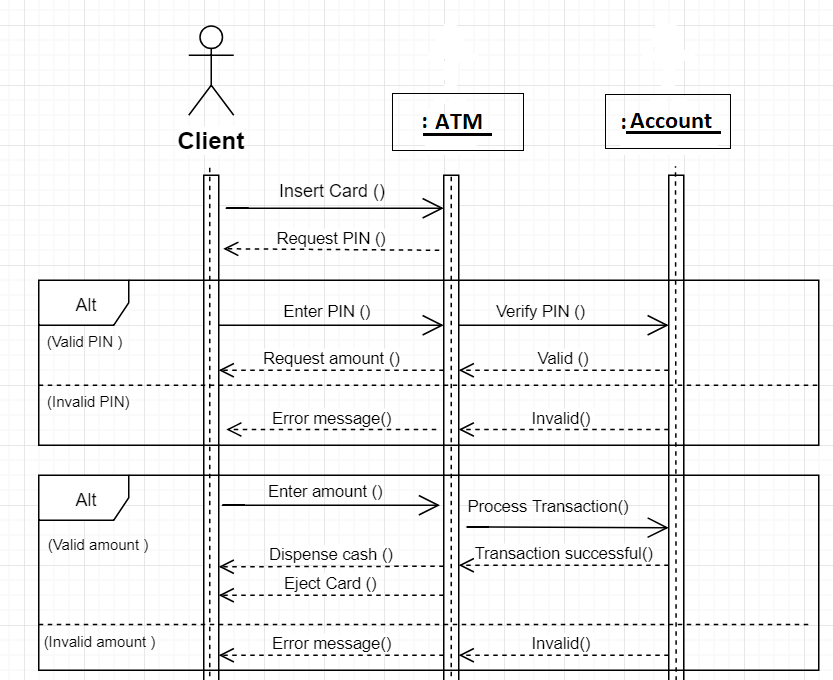
\includegraphics[width=\linewidth]{img/withdraw_sequence.png}
		\end{figure}

		\newpage\subsubsection{Collaboration Diagram}	
		\begin{figure}[h!]
		  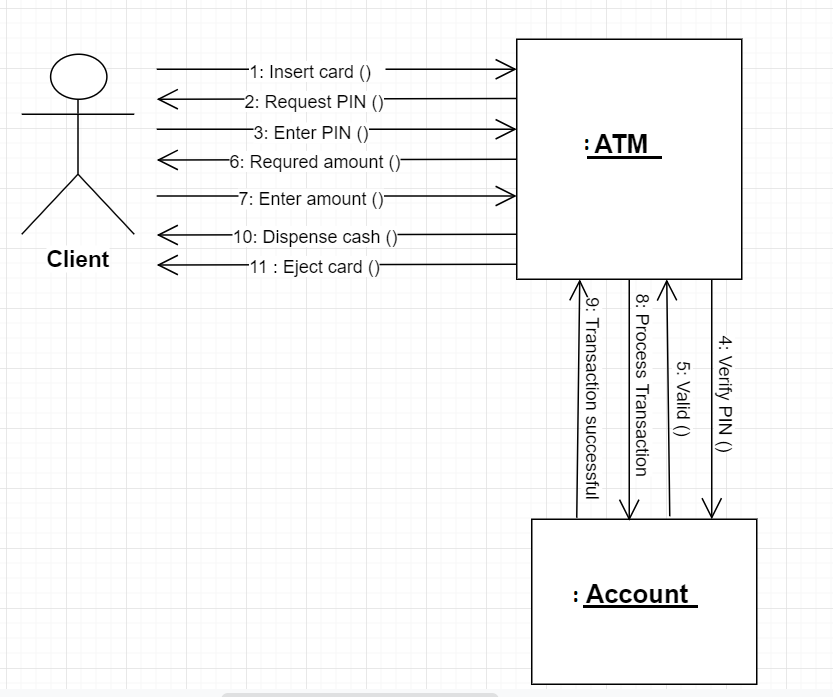
\includegraphics[width=\linewidth]{img/withdraw_collaboration.png}
		\end{figure}

		\newpage\subsubsection{Activity Diagram}
		\begin{figure}[h!]
			\begin{center}
				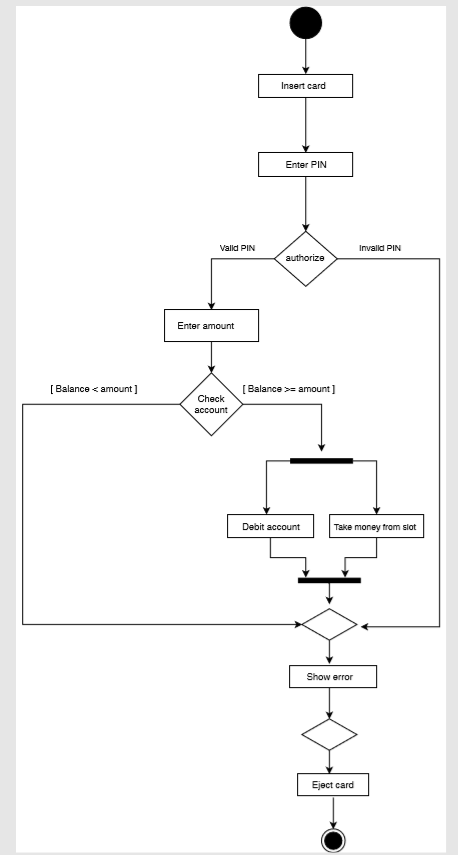
\includegraphics[height=\linewidth]{img/withdraw_activity.png}
			\end{center}
		\end{figure}

		\newpage\subsubsection{Flow Chart}
		\begin{figure}[h!]
			\begin{center}
				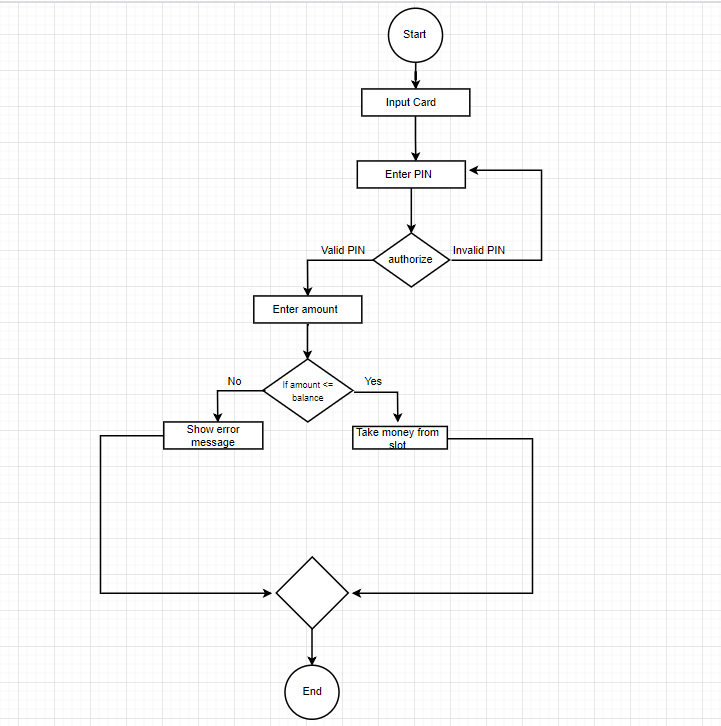
\includegraphics[height=\linewidth]{img/withdraw_flowchart.png}
			\end{center}
		\end{figure}
	\newpage\subsection{Deposit Money}
	\subsubsection{Use Case Scenario}
		\textbf{Use Case Name:}	Deposit money into account.
		\newline\textbf{Goal:} To deposit money (cash notes) into account.
		\newline\textbf{Actors:} user, Bank 	
		\newline\textbf{Precondition:} user is validated 	
		\newline\textbf{Primary Scenario:}	
			\begin{enumerate}[label*=\arabic*.]
				\item ATM screen displays menu.
			    \item The user presses on “Deposit”.
			    \item The machine displays a message to insert the notes into the allocated slot.
			    \item The user inserts the notes.
			    \item The machine verifies the notes.
			    \item The system displays the new balance value and sends it to the bank.
			    \item The bank adds the extra balance value to the old balance.
			    \item The user quits the session.
			    \item The ATM ejects the user’s card.
			\end{enumerate}
		\textbf{Variant:}\newline
			\hspace*{5mm}5a. The notes are not verified or accepted; the ATM ejects them.\newline
			\hspace*{5mm}*. The user might quit during any logical step; the ATM will eject the card.

		\newpage\subsubsection{Use Case Diagram}
			\begin{figure}[h!]
			  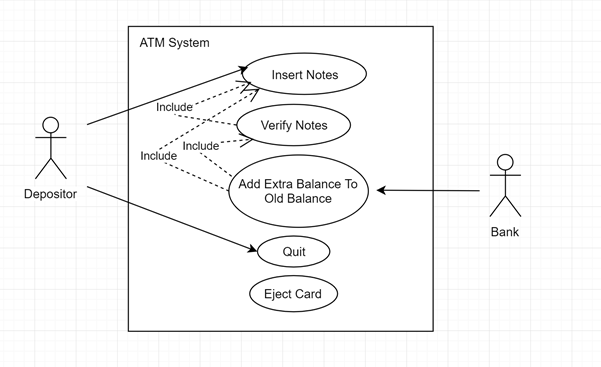
\includegraphics[width=\linewidth]{img/deposit_usecase.png}
			\end{figure}

		\newpage\subsubsection{Sequence Diagrams}
		\begin{figure}[h!]
		  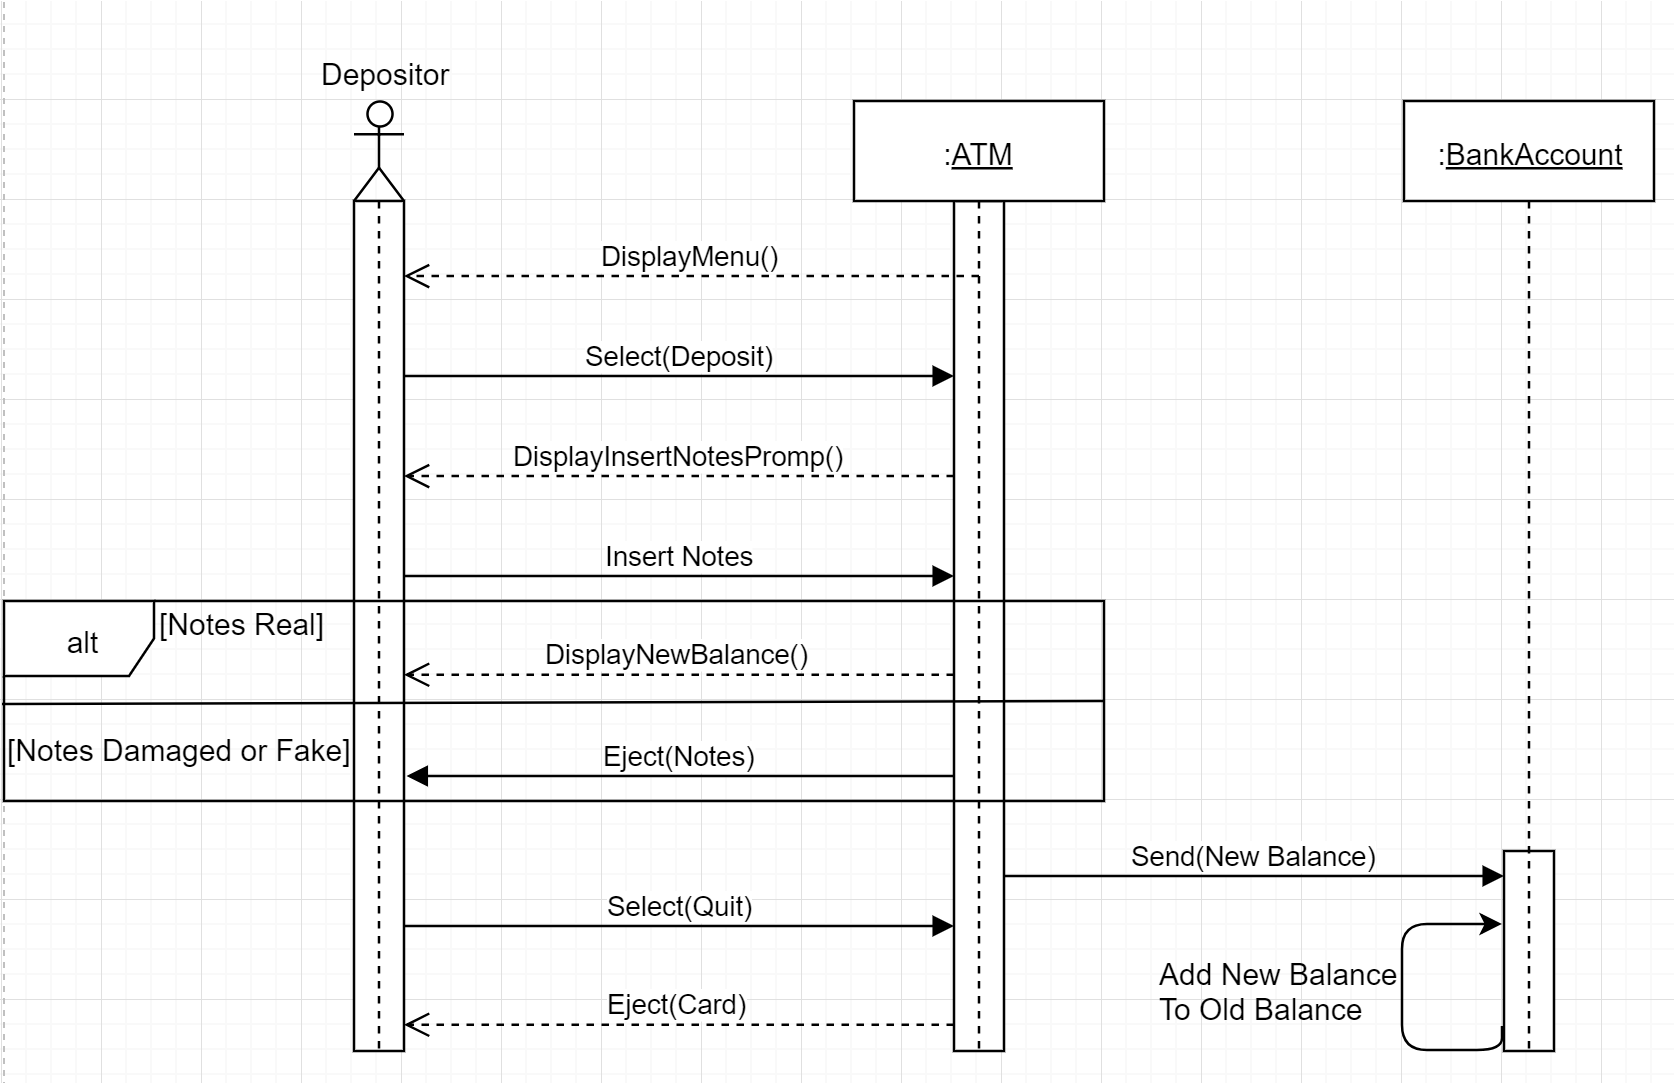
\includegraphics[width=\linewidth]{img/deposit_sequence.png}
		\end{figure}

		\newpage\subsubsection{Collaboration Diagram}	
		\begin{figure}[h!]
		  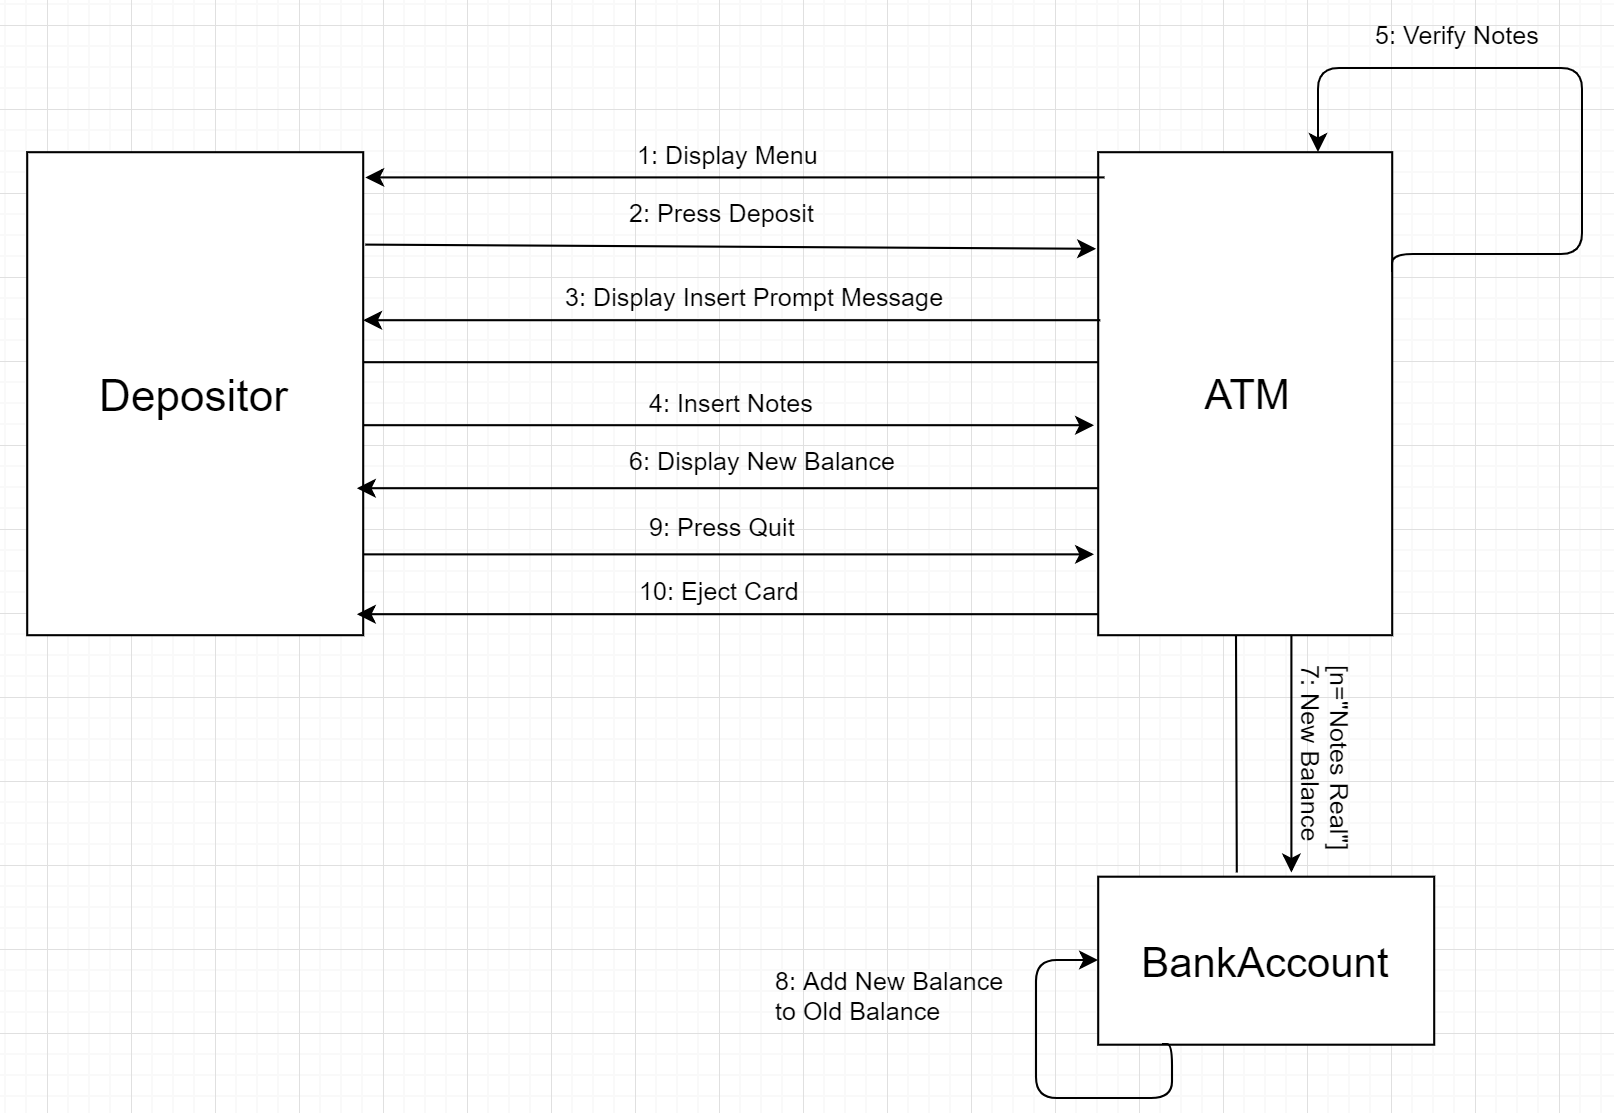
\includegraphics[width=\linewidth]{img/deposit_collaboration.png}
		\end{figure}

		\newpage\subsubsection{Activity Diagram}
		\begin{figure}[h!]
			\begin{center}
				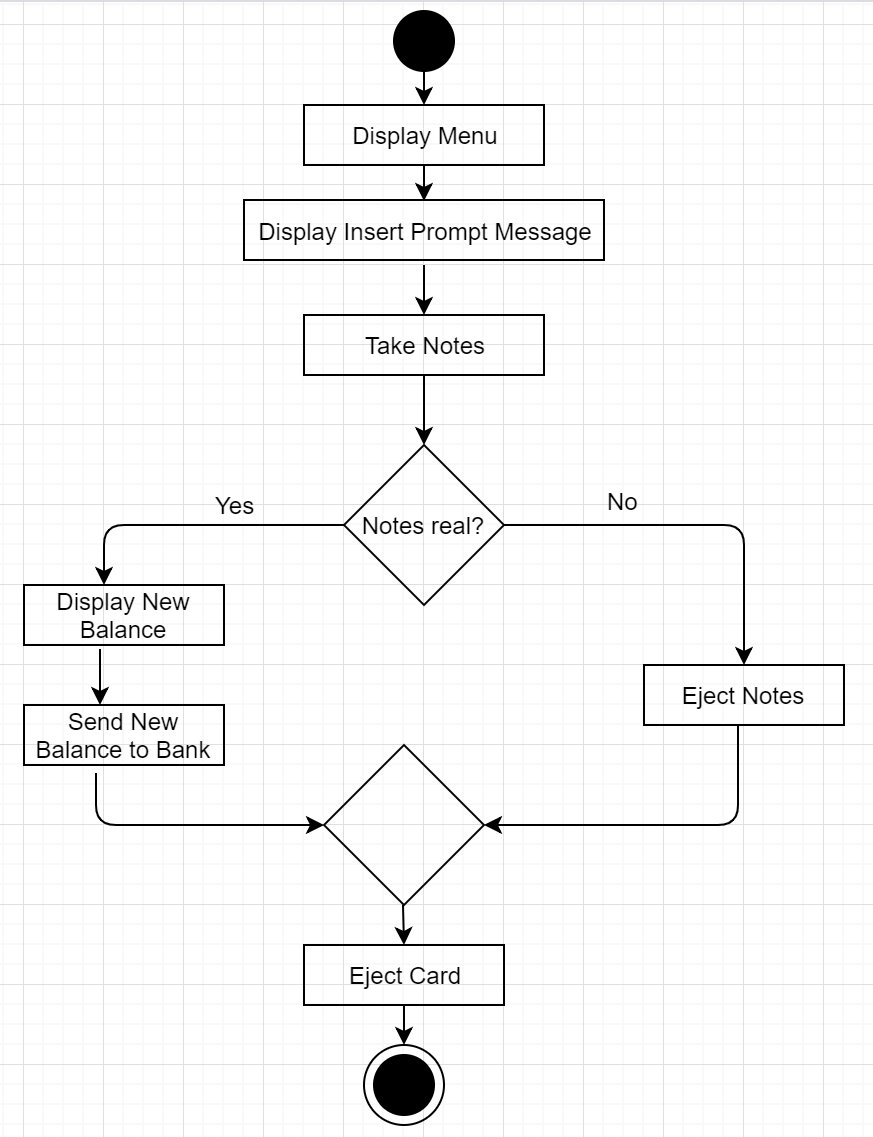
\includegraphics[height=\linewidth]{img/deposit_activity.png}
			\end{center}
		\end{figure}

		\newpage\subsubsection{Flow Chart}
		\begin{figure}[h!]
			\begin{center}
				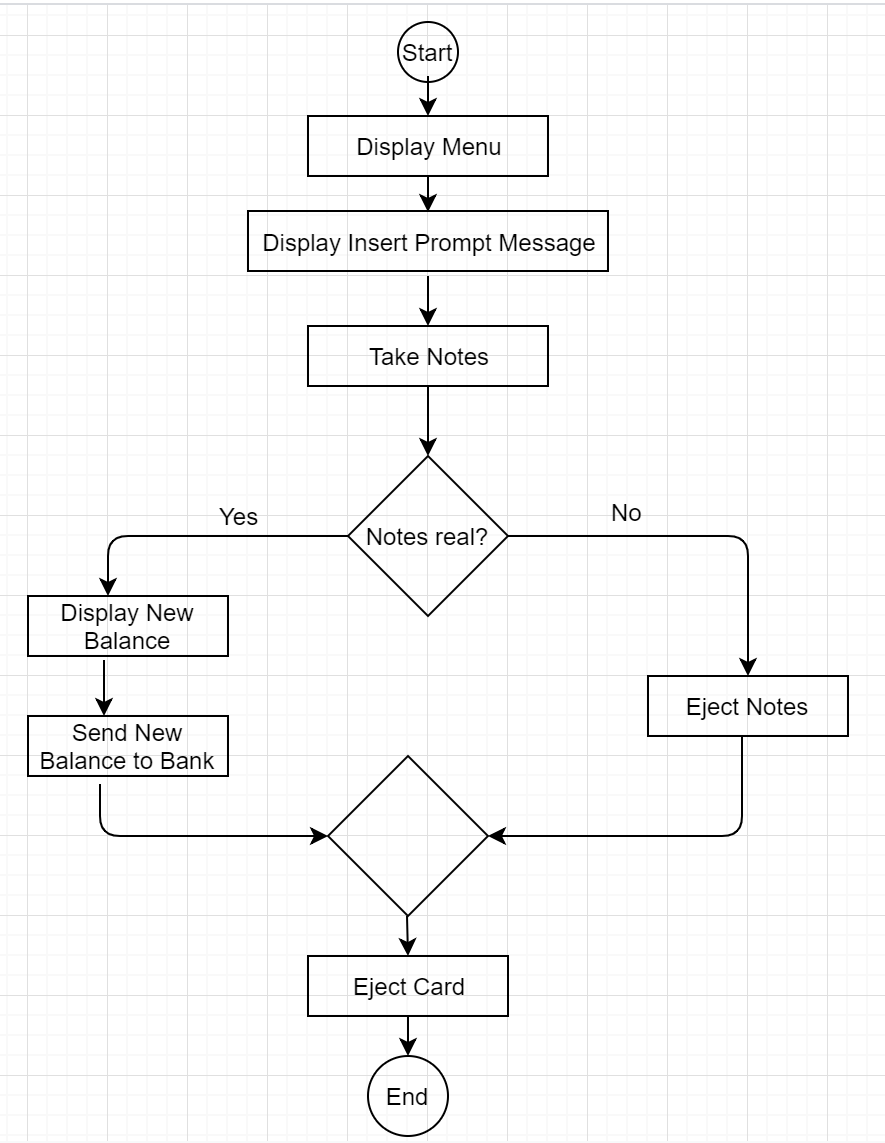
\includegraphics[height=\linewidth]{img/deposit_flowchart.png}
			\end{center}
		\end{figure}
	\newpage\subsection{Transfer}
		\subsubsection{Use Case Scenario}
		\textbf{Use Case Name:}	transfer money to another account.
		\newline\textbf{Goal:} to transfer money.
		\newline\textbf{Actors:} user, receiver, Bank 	
		\newline\textbf{Precondition:} user is validated 	
		\newline\textbf{Primary Scenario:}	
			\begin{enumerate}[label*=\arabic*.]
				\item ATM shows menu.
				\item user chooses "transfer money".
				\item ATM asks user to enter receiver's IBAN.
				\item If IBAN is correct, ATM asks for the amount transferred.
				\item If the amount is available in the user's account, money is transferred to receiver's account.
				\item User quits.
				\item ATM ejects the card.
			\end{enumerate}
		\textbf{Variant:}\newline	
			\hspace*{5mm}4a. If IBAN is incorrect, banks asks the user to enter it again.\newline
			\hspace*{5mm}5a. If the amount transferred is less than the user's current balance, the ATM shows an error message.\newline
			\hspace*{5mm}*. The user may cancel the session; the ATM ejects the card.

		\newpage\subsubsection{Use Case Diagram}
			\begin{figure}[h!]
			  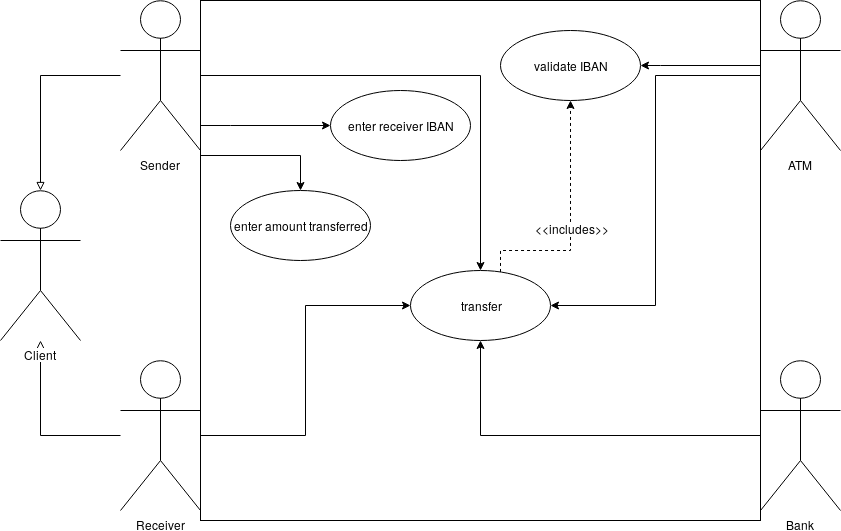
\includegraphics[width=\linewidth]{img/transfer_usecase.png}
			\end{figure}

		\newpage\subsubsection{Sequence Diagrams}
		\begin{figure}[h!]
		  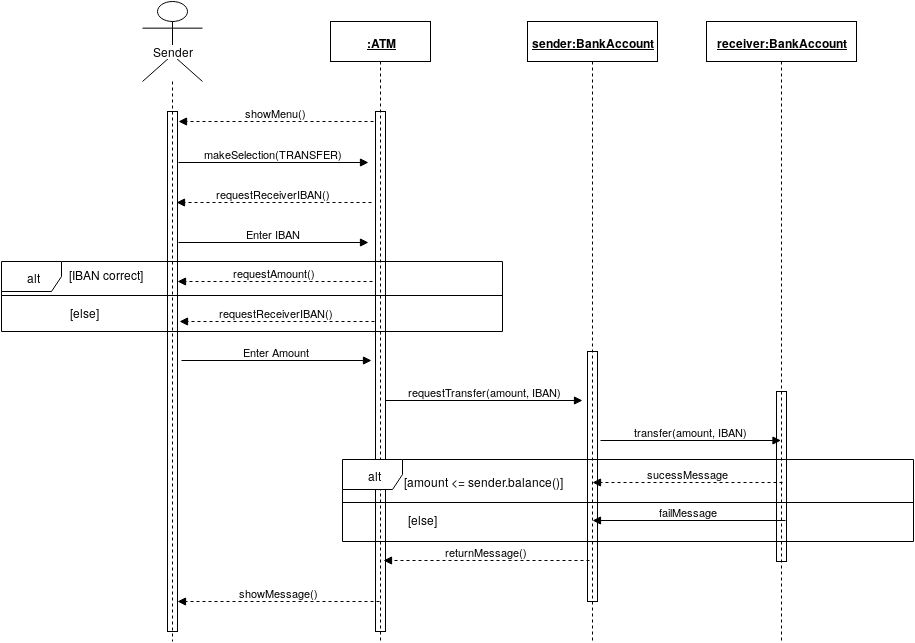
\includegraphics[width=\linewidth]{img/transfer_sequence.png}
		\end{figure}

		\newpage\subsubsection{Collaboration Diagram}	
		\begin{figure}[h!]
		  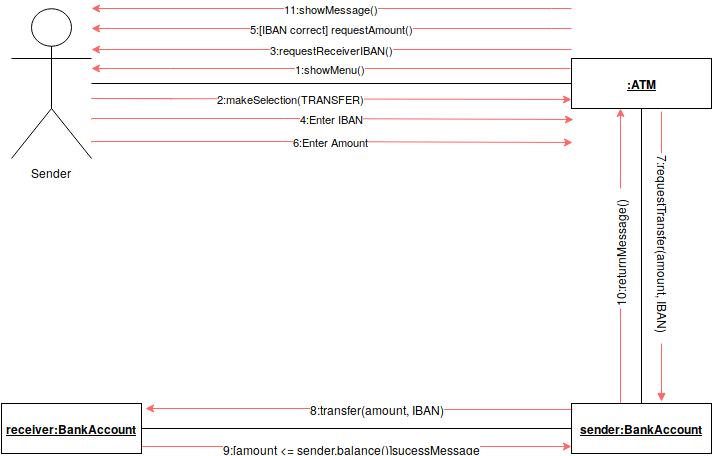
\includegraphics[width=\linewidth]{img/transfer_collaboration.png}
		\end{figure}

		\newpage\subsubsection{Activity Diagram}
		\begin{figure}[h!]
			\begin{center}
				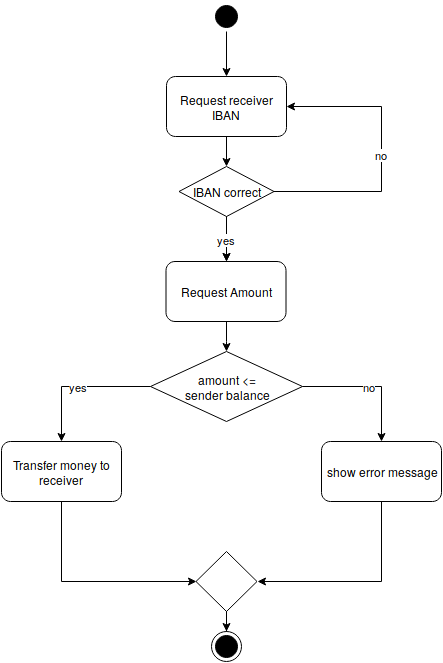
\includegraphics[height=\linewidth]{img/transfer_activity.png}
			\end{center}
		\end{figure}

		\newpage\subsubsection{Flow Chart}
		\begin{figure}[h!]
			\begin{center}
				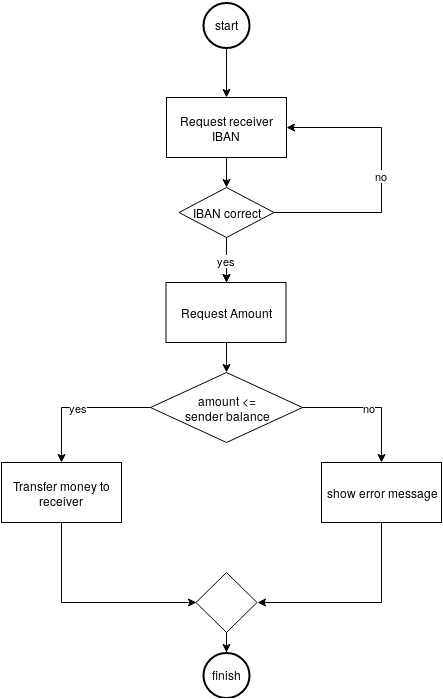
\includegraphics[height=\linewidth]{img/transfer_flowchart.png}
			\end{center}
		\end{figure}
	\newpage\subsection{For The Whole System}
	\subsubsection{Context Diagram}
		\begin{figure}[h!]
			\begin{center}
				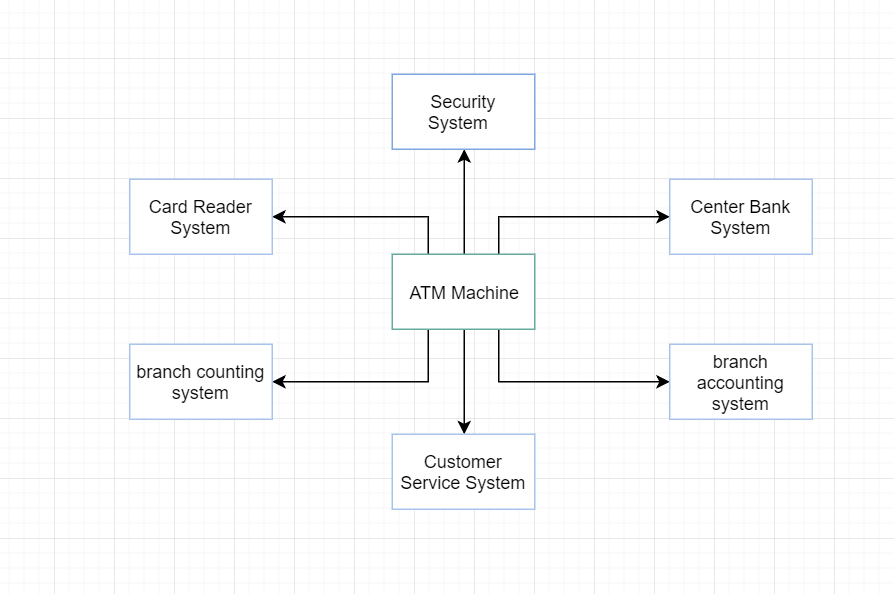
\includegraphics[width=\linewidth]{img/context.png}
			\end{center}
		\end{figure}	
	\newpage\subsubsection{Use-case Diagram}
		\begin{figure}[h!]
			\begin{center}
				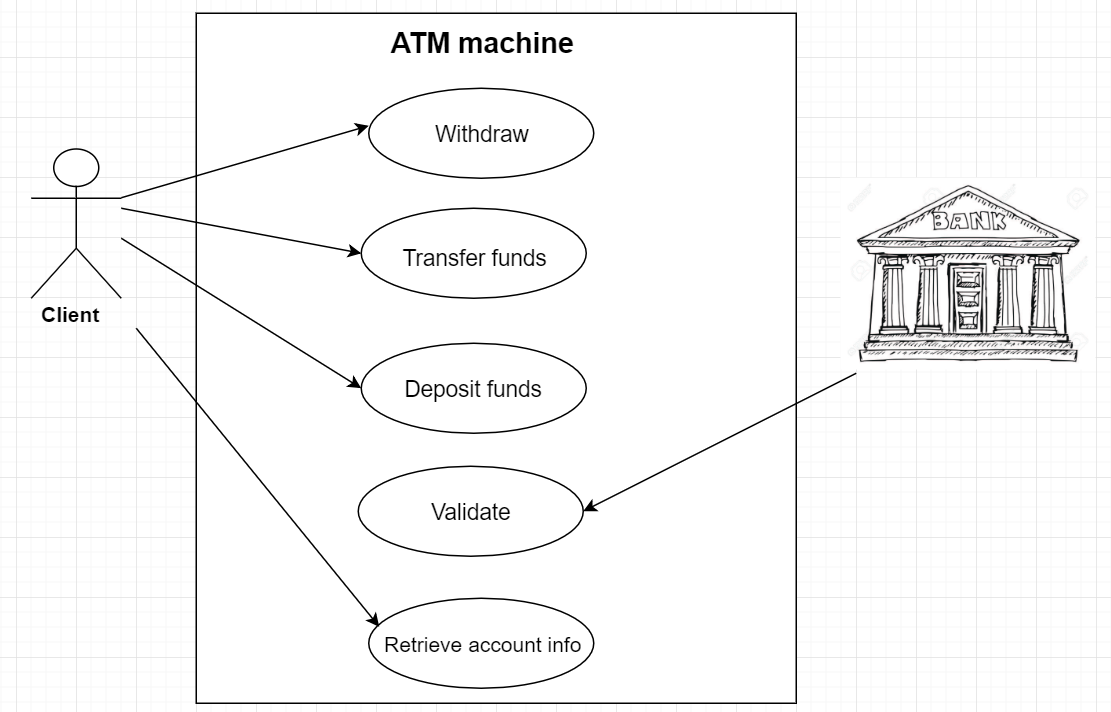
\includegraphics[width=\linewidth]{img/usecase.png}
			\end{center}
		\end{figure}
	\newpage\subsubsection{Component diagram}
		\begin{figure}[h!]
			\begin{center}
				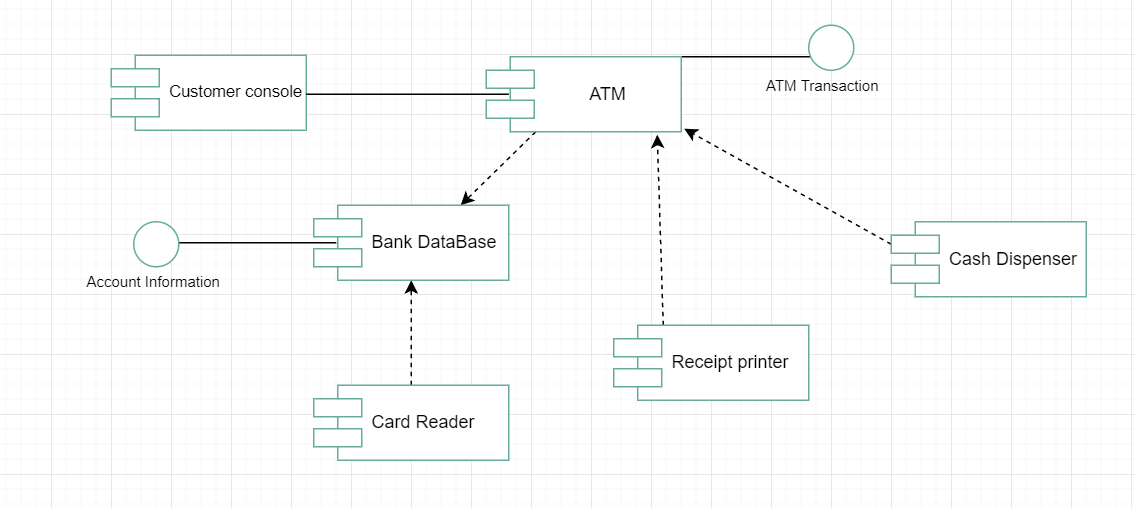
\includegraphics[width=\linewidth]{img/component.png}
			\end{center}
		\end{figure}
	\newpage\subsubsection{Deployment diagram}
		\begin{figure}[h!]
			\begin{center}
				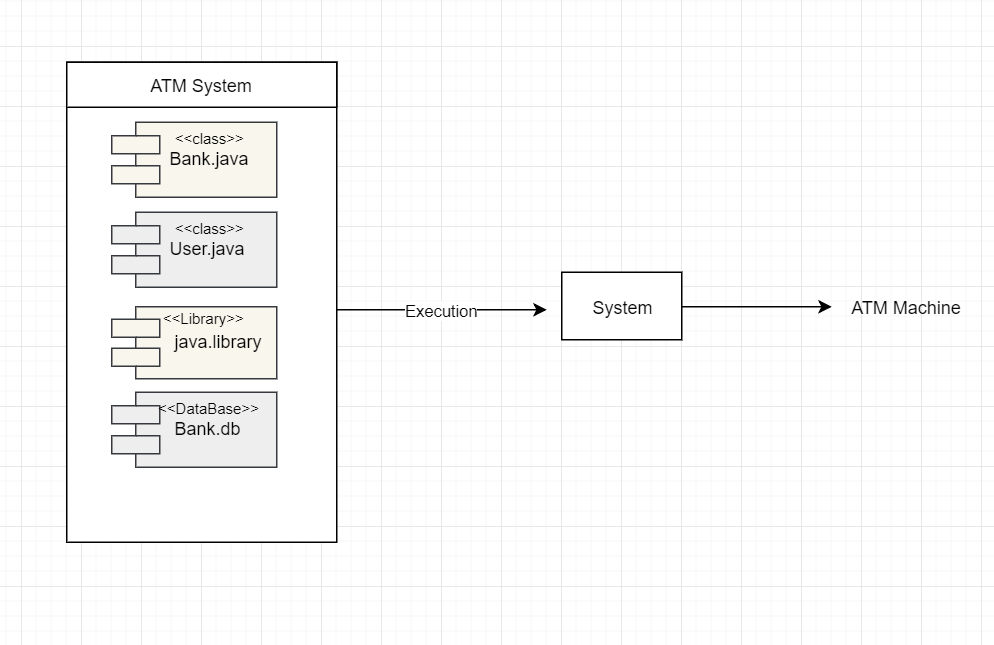
\includegraphics[width=\linewidth]{img/deployment.png}
			\end{center}
		\end{figure}
	\newpage\subsubsection{Data flow Diagram}	
		\begin{figure}[h!]
			\begin{center}
				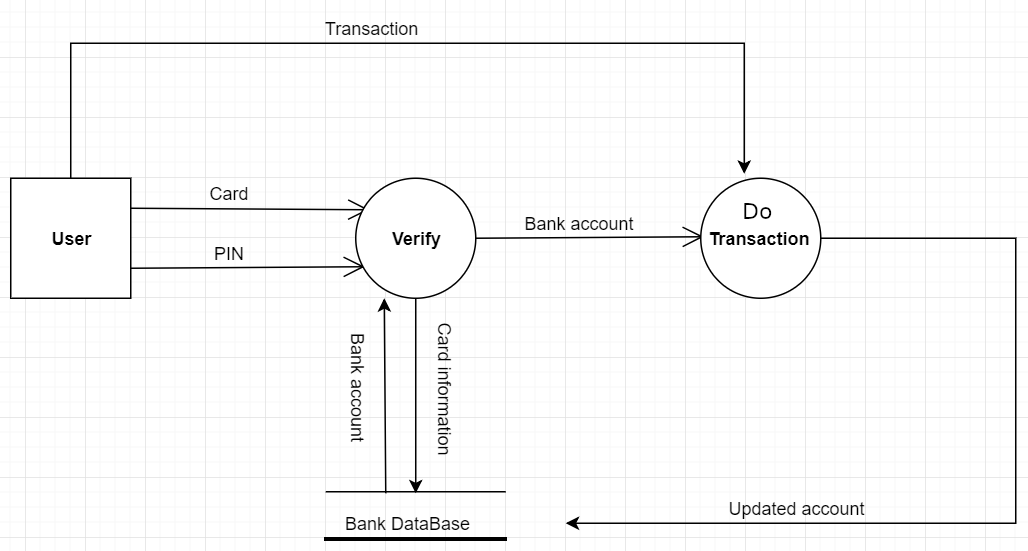
\includegraphics[width=\linewidth]{img/dataflow.png}
			\end{center}
		\end{figure}	
	\newpage\subsubsection{Class Diagram}
		\begin{figure}[h!]
			\begin{center}
				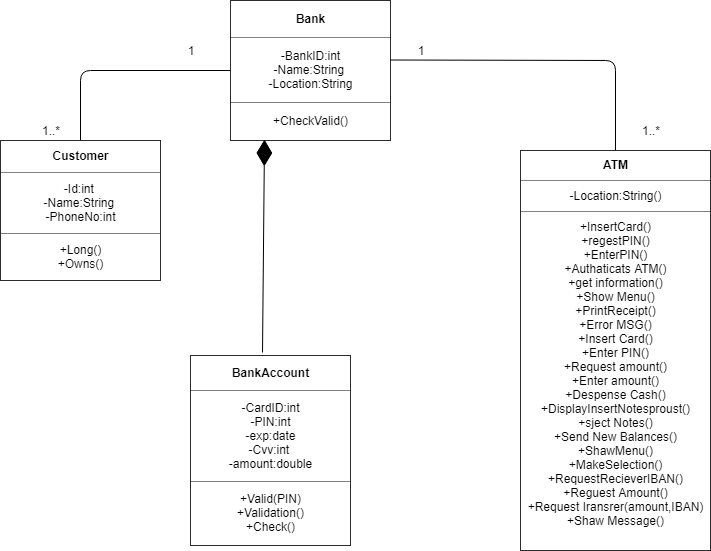
\includegraphics[width=\linewidth]{img/class.png}
			\end{center}
		\end{figure}
	\newpage\subsubsection{Object Diagram}		
		\begin{figure}[h!]
			\begin{center}
				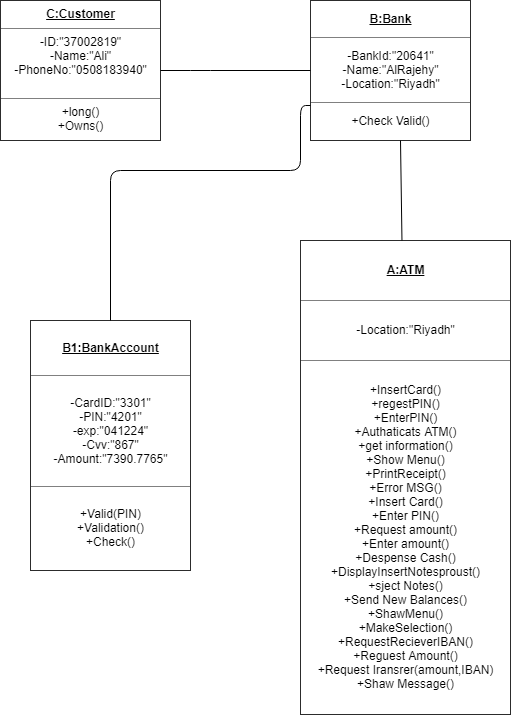
\includegraphics[width=\linewidth]{img/object.png}
			\end{center}
		\end{figure}
	\newpage\subsubsection{Architectural patterns}
		\paragraph{} The architecture pattern used is pipe and filter, since the system is mainly data processing and focus on updating the database.
		\begin{figure}[h!]
			\begin{center}
				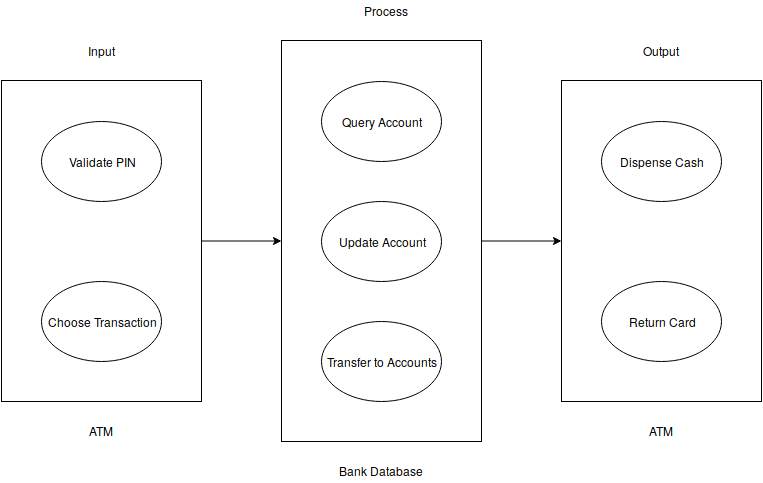
\includegraphics[width=\linewidth]{img/architecture.png}
			\end{center}
		\end{figure}


	\newpage
	\addcontentsline{toc}{section}{References}
	\bibliographystyle{ieeetr}
	\bibliography{References}


\end{document}
